\documentclass[journal,12pt,twocolumn]{IEEEtran}
\IEEEoverridecommandlockouts
\usepackage{cite}
\usepackage{amsmath,amssymb,amsfonts,bm}
\usepackage{mathtools}
\usepackage{tkz-euclide} 
\usetikzlibrary{calc,math}
 \usepackage{caption}
\usepackage{listings}
\let\vec\mathbf
%\newcommand{\myvec}[1]{\ensuremath{\begin{pmatrix}#1\end{pmatrix}}}
%\newcommand{\norm}[1]{\left\lVert#1\right\rVert}
%\lstset{
%frame=single, 
%breaklines=true,
%columns=fullflexible
%}
\begin{document}

\title{Matrix Theory EE5609 - Assignment 3\\
Find if a triangle is isosceles triangle.
}

\author{\IEEEauthorblockN{Sandhya Addetla}\\
\IEEEauthorblockA{PhD Artificial Inteligence Department} \\
23-Sep-2020\\
AI20RESCH14001\\
 }

\maketitle
\begin{abstract}
This document provides a solution for finding if a traingle is isosceles given two equal altitudes of the triangle
\end{abstract}
%
%Download all python codes from 
%\begin{lstlisting}
%https://github.com/SANDHYA-A/Codes/blob/master/Assignment2.py
%\end{lstlisting}


\section{Problem Statement}
BE and CF are two equal altitudes of a triangle ABC. Using RHS congruence rule, prove that the triangle ABC is isosceles.

\section{Theory}
By RHS theorem, in two right-angled triangles, if the length of the hypotenuse and one side of one triangle, is equal to the length of the hypotenuse and corresponding side of the other triangle, then the two triangles are congruent.

\captionsetup{justification=centering}

\begin{figure}[!h]
\centering
%\includegraphics[width=0.7\columnwidth]{
\resizebox{.5\columnwidth}{!}{
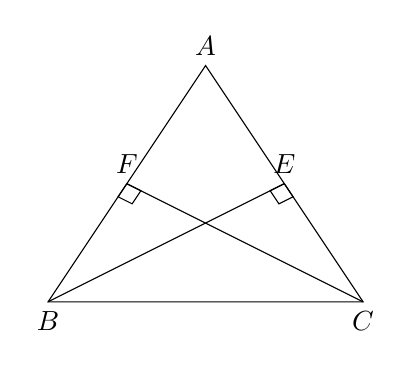
\begin{tikzpicture} 
        \coordinate (A) at (2, 3) {};
        \coordinate (B) at (0, 0) {};
        \coordinate (C) at (4, 0) {};
        \coordinate (F) at (1, 1.5) {};
        \coordinate (E) at (3, 1.5) {};
\draw (A)node[above]{$A$}--(B)node[below]{$B$}--(C)node[below]{$C$}--cycle;
\draw (B)node[below]{}--(E)node[above]{$E$};
\draw (C)node[below]{}--(F)node[above]{$F$};
\tkzMarkRightAngle[size=.2](B,E,C);
\tkzLabelAngle[dist=.5](B,E,C){};
\tkzMarkRightAngle[size=.2](C,F,B);
\tkzLabelAngle[dist=.5](C,F,B){};
\end{tikzpicture}
}
\caption{Triangle with equal altitudes on two sides}
\label{myfig}
\end{figure}
\section{Solution}
Consider the two triangles $\triangle{AFC}$ and $\triangle{ABE}$. We can observe that vertex A is common to both the traingles and the angle between the sides $\angle{BAE}$ and $\angle{FAC}$ are same.
Let the two equal altitudes of the triangle be \textit l
\begin{align}
\angle{BAE} = \angle{FAC}\\
\sin\theta = \sin\theta\\
\frac{BE}{BA}= \frac{CF}{CA} 
\end{align} 
We know that the altitudes BE and CF are equal

Hence we obtain
\begin{align}
\frac{\textit l}{BA}= \frac{\textit l}{CA} \\
\therefore BA = CA
\end{align}
Hence the  $\triangle{ABC}$ is an isosceles triangle with sides BA and CA of equal length.
\end{document}